\documentclass{article}

\usepackage[margin=1in]{geometry}

\usepackage{math}
\usepackage{algorithm, algpseudocode}
\usepackage{graphicx}

\DeclareMathOperator{\argmin}{argmin}
\DeclareMathOperator{\mspin}{MSPIN}

\numberwithin{equation}{section}

\title{Phase-field fracture models and MSPIN} % nb: placeholder
\author{Conor McCoid \and Blaise Bourdin}

\begin{document}

\maketitle

\begin{abstract}
---
\end{abstract}

\section{Introduction}
\label{sec: intro}

Brittle fracture is the sudden nucleation and propagation of cracks in otherwise elastic material.
This type of damage can be catastrophic in applications such as civil engineering or crystal growth.
Because brittle fracture occurs so rapidly, it is difficult to model the phenomenon with standard calculus.
Instead, Francfort and Marigo (nb: cite) propose using a variational principle: the vector field of the displacement of the material minimizes an energy potential that combines elastic forces and the Griffiths energy of all cracks (nb: cite Griffith?).

This variational approach then requires calculating the Griffith's energy, a challenge in practice.
As an approximation, one introduces a phase-field variable, a scalar field representing the damage in the material.
In this phase-field model, one seeks to find both the displacement and damage that minimizes the approximation to the energy potential.

The energy potential is non-convex, making optimization difficult.
The solution to this has been alternate minimization, holding either damage or displacement constant while updating the other.
When either field is kept fixed, the energy potential is convex in the other, meaning by solving two sequential convex optimization problems one arrives at an iterative method for solving the problem.
This process is costly when the crack nucleates, requiring several orders of magnitude more iterations to find a solution.

[Recent advances]
In (nb: cite 3K), the authors applied the multiplicative Schwarz preconditioning inexact Newton method (MSPIN) to the phase-field model.

In this paper, we propose to combine alternate minimization with MSPIN to minimize the energy potential over a 2D or 3D subspace of the degrees of freedom by finding the minimum of polynomial interpolants.
These interpolants are based on P2 finite elements.
By using both alternate minimization and MSPIN, the search space for backtracking is higher dimensional and is guaranteed to give lower energy potentials than either method on their own.

In Section \ref{sec: bg}, we cover necessary background information, including a description of the phase-field model and algorithms from previous works.
In Section \ref{sec: interpolant}, we introduce the polynomial interpolants, how to minimize them, and when this minimization may fail.
In Section \ref{sec: num}, we compare the various methods applied to numerical examples.

\section{Background}
\label{sec: bg}

A given brittle material has inherent elastic properties: a critical energy release rate $G_c$, and a stiffness tensor $A$.
The material occupies a domain $\Omega \subset \bbr^n$ and is subjected to a set of boundary conditions, such as specifying the displacement on part of the boundary.
The variational approach to fracture seeks to minimize the energy potential
\begin{equation} \label{eq: var}
	E(\vec{u}, \Gamma) := \int_{\Omega \setminus \Gamma} \frac{1}{2} A \epsilon(\vec{u}) \cdot \epsilon(\vec{u}) dx + G_c \mathcal{H}^{n-1}(\Gamma),
\end{equation}
where $\vec{u}$ is the vector field denoting the displacement of the material,
$\Gamma$ defines all cracks in the material, $\mathcal{H}^{n-1}(\Gamma)$ is its $(n-1)$-dimensional Hausdorff measure, and $\epsilon(\vec{u})$ is the symmetrized gradient of $\vec{u}$:
\begin{equation*}
	\epsilon(\vec{u}) := \frac{1}{2} \left ( \nabla \vec{u} + \nabla^\top \vec{u} \right ).
\end{equation*}

Computing the Hausdorff measure of the unknown crack $\Gamma$ is untenable in practice.
Instead, one introduces a phase-field scalar field $v : \Omega \to [0,1]$ called damage, which is intended to represent $\Gamma$:
at the crack, $v$ should equal 1, while away from the crack, $v$ should equal 0.
This requires introducing a regularization length $\ell>0$.
The phase-field energy may be expressed as
\begin{equation} \label{eq: energy} % nb: fix this
	E_\ell(\vec{u}, v) = \int_{\Omega} \frac{a(v) + k_\ell}{2} A \epsilon(\vec{u}) \cdot \epsilon(\vec{u}) dx + \frac{G_c}{4 c_\omega} \int_{\Omega} \left ( \frac{\omega(v)}{\ell} + \ell \abs{\nabla v}^2 \right ) dx,
\end{equation}
where $a(v)$ and $\omega(v)$ are continuous monotonic functions satisfying
\begin{equation*}
	a(0)=0, \quad a(1)=1, \quad \omega(0)=1, \quad \omega(1)=0, \quad c_\omega := \int_0^1 \sqrt{\omega(s)} ds,
\end{equation*}
and $k_\ell$ is a constant smaller than $\ell$.
In this article, we will use the AT2 model:
\begin{equation} \label{eq: AT2}
	a(v) = (1-v)^2, \quad \omega(v) = v^2, \quad c_\omega = \frac{1}{2}.
\end{equation}

In addition to boundary conditions, the quasi-static phase-field model is constrained by an irreversibility condition on the damage scalar field.
As time moves forward, damage to the material can only increase; the material cannot heal itself.
At each time step, the damage field is saved as the new lower bound on the constraints:
\begin{equation*}
	v(t_{i-1}) \leq v(t_i) \leq 1, \quad \forall x \in \Omega.
\end{equation*}
Care must be taken to enforce this condition.

\subsection{Alternate Minimization}
\label{subsec: altmin}

The energy potential $E_\ell(\vec{u},v)$, see \eqref{eq: energy}, is not convex.
However, it is convex in both $\vec{u}$ and $v$ separately.
This then leads to the idea for alternate minimization: hold $v$ constant while solving for $\vec{u}$, then hold $\vec{u}$ constant at its new solution while solving for $v$.
Algorithm \ref{alg: altmin} gives the alternate minimization algorithm for a given time step.
\begin{algorithm}
	\caption{AltMin \\
		$\vec{u}_0$: initial displacement, $v_0$: initial damage, $\tau$: tolerance}
	\begin{algorithmic}[1]
	\State Find $\vec{u}_1 := \argmin_u E_\ell(\vec{u}, v_0)$, subject to boundary conditions
	\State Find $v_1 := \argmin_v E_\ell(\vec{u}_1, v)$, subject to boundary and irreversibility conditions
	\While{$\norm{v_1 - v_0} > \tau$}
		\State $v_0 \gets v_1$, $\vec{u}_0 \gets \vec{u}_1$
		\State Find $\vec{u}_1 := \argmin_u E_\ell(\vec{u}, v_0)$, subject to boundary conditions
		\State Find $v_1 := \argmin_v E_\ell(\vec{u}_1, v)$, subject to boundary and irreversibility conditions
	\EndWhile
	\end{algorithmic}
	\label{alg: altmin}
\end{algorithm}
Because solving for damage includes irreversibility conditions, damage is found using a variational inequality Newton's method.
Displacement may be found with any linear solver.

AltMin may be viewed as a field-split multiplicative Schwarz method.
The two `fields' of damage and displacement are treated separately and sequentially.
This allows the use of some of the techniques reserved for Schwarz methods to be applied here.
In particular, in Section \ref{subsec: mspin} we will examine applying MSPIN to the problem.

\subsection{Active set methods}
\label{subsec: as}

As described above, the damage scalar field is subject to a variational inequality that changes at each time step:
\begin{equation*}
	v(t_{i-1}) \leq v(t_i) \leq 1, \quad \forall x \in \Omega.
\end{equation*}
In Section \ref{subsec: altmin}, this is said to be handled by a variational inequality Newton's method, or VINewton, which uses an active set method.

Active set methods separate all degrees of freedom into two sets: an active set, where the constraints are met or exceeded, and an inactive set, where the constraints remain intact, i.e.
\begin{align*}
	\Omega_{\text{active}} & := \Set{x \in \Omega}{v(t_i) \leq v(t_{i-1}) \lor v(t_i) \geq 1},
	\\ \Omega_{\text{inactive}} & := \Set{x \in \Omega}{v(t_{i-1}) < v(t_i) < 1}.
\end{align*}
For degrees of freedom in the active set, the value of the scalar field is set to the closest bound.
If $v(t_i) \leq v(t_{i-1})$, then $v(t_i) \gets v(t_{i-1})$.
For degrees of freedom in the inactive set, one tests whether the change caused by adding the new Newton direction would violate the constraints.
If so, the value is set to the closest bound and the degree of freedom is moved to the active set.
If not, then the method is allowed to proceed as a standard Newton's method.

\subsection{MSPIN}
\label{subsec: mspin}

Multiplicative Schwarz preconditioning inexact Newton (MSPIN) was first described in (nb: cite Cai and Keyes), with further explanation for field-split Schwarz methods in (nb: cite Liu and Keyes).
MSPIN has been previously applied to phase-field fracture models in (nb: cite 3K).
There, the authors used cubic backtracking to globalize the Newton direction, see Section \ref{subsec: cb} below.
Note that their model differs slightly from the one presented here.

To describe MSPIN, we must first present AltMin as a multiplicative Schwarz method.
The Jacobian of the phase-field energy is
\begin{equation} \label{eq: jacobian}
	J := \begin{bmatrix} E_{uu} & E_{uv} \\ E_{vu} & E_{vv} \end{bmatrix}, \quad E_{xy} = \ddxy{E_\ell}{x}{y}.
\end{equation}
A single step of AltMin can then be thought of as solving the following nonlinear system:
\begin{equation*}
	\begin{bmatrix} E_{uu} \\ E_{vu} & E_{vv} \end{bmatrix} \begin{bmatrix} \vec{u}_1 \\ v_1 \end{bmatrix} = \begin{bmatrix} ~ & E_{uv} \\ & ~ \end{bmatrix} \begin{bmatrix} \vec{u}_0 \\ v_0 \end{bmatrix},
\end{equation*}
with additional blocks to represent boundary conditions, subject to the irreversibility condition.

The goal of MSPIN is to apply inexact Newton's method to a linearization of this system.
That is, MSPIN seeks to minimize
\begin{equation*}
	\vec{q} := \begin{bmatrix} \vec{u}_1 \\ v_1 \end{bmatrix} - \begin{bmatrix} \vec{u}_0 \\ v_0 \end{bmatrix}.
\end{equation*}
In (nb: cite Cai and Keyes, Liu and Keyes, and/or 3K), the Jacobian for this inexact Newton's method is shown to be
\begin{equation*}
	J_{\mspin} := \begin{bmatrix} E_{uu} \\ E_{vu} & E_{vv} \end{bmatrix}^{-1} \begin{bmatrix} E_{uu} & E_{uv} \\ E_{vu} & E_{vv} \end{bmatrix}
	= \begin{bmatrix} I \\ & E_{vv}^{-1} \end{bmatrix} \begin{bmatrix} I \\ -E_{vu} & I \end{bmatrix} \begin{bmatrix} E_{uu}^{-1} \\ & I \end{bmatrix} J.
\end{equation*}

The Newton direction proposed by MSPIN is the approximate solution to the system
\begin{equation} \label{eq: inexact newton}
	J_{\mspin} \vec{p} = \vec{q}.
\end{equation}
Since only an approximation is required, one can be found with a few iterations of a Krylov subspace method.
Note that both $E_{uu}$ and $E_{vv}$ have been inverted as part of the AltMin process.
Storing factorizations for these matrices can significantly speed up their use here, where each will need to be applied once per Krylov iteration.

We present MSPIN as applied to AltMin.
\begin{algorithm}
	\caption{MSPIN on AltMin \\
		$\vec{u}_0$: initial displacement, $v_0$: initial damage, $\tau$: tolerance}
	\begin{algorithmic}[1]
	\State Find $\vec{u}_1 := \argmin_u E_\ell(\vec{u}, v_0)$, subject to boundary conditions
	\State Find $v_1 := \argmin_v E_\ell(\vec{u}_1, v)$, subject to boundary and irreversibility conditions
	\While{$\norm{v_1 - v_0} > \tau$}
		\State $v_0 \gets v_1$, $\vec{u}_0 \gets \vec{u}_1$
		\State Find $\vec{u}_1 := \argmin_u E_\ell(\vec{u}, v_0)$, subject to boundary conditions
		\State Find $v_1 := \argmin_v E_\ell(\vec{u}_1, v)$, subject to boundary and irreversibility conditions
		\State Approximate the solution to eq. \eqref{eq: inexact newton}
		\State (optional) Apply globalization techniques
		\State Project solution onto the active set
	\EndWhile
	\end{algorithmic}
	\label{alg: mspin}
\end{algorithm}

\subsection{Cubic Backtracking}
\label{subsec: cb}

Many applications of Newton's method require globalization techniques to achieve convergence when starting away from the minimum.
When the Newton direction overshoots the minimum, these globalization techniques should search for a minimum between the starting point and the destination, usually through a line search.

Cubic backtracking (nb: cite) performs this line search by repeatedly interpolating cubic polynomials and finding their minima.
Note that a cubic polynomial interpolant requires four pieces of information, but Newton's method only provides three:
the value of the function at the starting point, $f(\vec{x})$;
the value of the function in the Newton direction, $f(\vec{x} + \vec{p})$, and;
the derivative of the function in the Newton direction, $\vec{p} \cdot \nabla f(\vec{x})$.

To get a fourth piece of information, first form a quadratic interpolant with this information.
Find the minimum of this polynomial and test the value of the function there, thus getting enough information for a cubic polynomial.
If the function is smaller at this point, then this ends the line search.
Otherwise, find the minimum of the cubic interpolant and repeat.
This algorithm is summarized in Algorithm \ref{alg: cb}.
\begin{algorithm}
	\caption{Cubic backtracking (nb: cite) \\
		$p$: search direction, $x$: current position, $f$: objective function, $\alpha$: bound on step size, $\tau$: tolerance (nb: of some kind, check)}
	\begin{algorithmic}[1]
	\State Calculate $c = p^\top \nabla f(x)$
	\If{$f(x + p) \leq f(x) + \alpha c$}
		\State Set $\lambda = 1$
	\ElsIf{$\norm{p} \leq \tau$}
		\State (nb: check)
	\Else
		\State Find $\lambda$ such that $x + \lambda p$ minimizes the degree 2 polynomial interpolating $f(x)$, $f(x + p)$, and $g$: $$\lambda = -c / \left ( 2\left ( f(x+p) - f(x) - c \right ) \right )$$
		\State Set $\lambda_0=1$, $\lambda_1 = \lambda$
		\While{$f(x + \lambda p) > f(x) + \alpha \lambda c$}
			\State Find the coefficients of the degree 3 polynomial interpolating $f(x)$, $f(x + \lambda_0 p)$, $f(x + \lambda_1 p)$, and $g$: $$\begin{bmatrix} a \\ b \end{bmatrix} = \frac{1}{\lambda_1 - \lambda_0} \begin{bmatrix} 1/\lambda_1^2 & -1/\lambda_0^2 \\  -\lambda_0/\lambda_1^2 & \lambda_1/\lambda_0^2 \end{bmatrix} \begin{bmatrix} f(x+\lambda_1 p) - f(x) - \lambda_1 c \\ f(x+\lambda_0 p) - f(x) - \lambda_0 c \end{bmatrix}$$
			\If{$a=0$}
				\State $\lambda = -c / 2b$
			\Else
				\State $\lambda = \frac{-b + \sqrt{b^2 - 3a c}}{3a}$
			\EndIf
			\If{$\lambda > 0.5 \lambda_1$}
				\State $\lambda = 0.5 \lambda_1$
			\EndIf
			\State $\lambda_0 = \lambda_1$, $\lambda_1 = \lambda$
		\EndWhile
	\EndIf
	\State Return $\lambda$, amount to travel in search direction $p$ to minimize $f(x)$
	\end{algorithmic}
	\label{alg: cb}
\end{algorithm}

\section{Interpolant minimization}
\label{sec: interpolant}

When using MSPIN, one has two potential directions for minimization: the AltMin direction $\vec{q}$ and the Newton direction $\vec{p}$.
Let's try using both while applying similar ideas to cubic backtracking.
Rather than find the minimum of a single variable cubic polynomial, find the minimum of a multivariate quadratic polynomial interpolant.
Here we present three options for interpolants to minimize.

\subsection{Parallelogram}
\label{subsec: para}

We begin by considering a 2D interpolant using the AltMin and Newton directions, $\vec{q}$ and $\vec{p}$.
For this interpolant, we need six pieces of information.
Five are provided by MSPIN:
the value of the function at the starting point, $f(\vec{x})$;
the value of the function in the AltMin direction, $f(\vec{x} + \vec{q})$;
the value of the function in the Newton direction, $f(\vec{x} + \vec{p})$;
the derivative of the function in the AltMin direction, $\vec{q} \cdot \nabla f(\vec{x})$, and;
the derivative of the function in the Newton direciton, $\vec{p} \cdot \nabla f(\vec{x})$.

One choice for a sixth piece of information is the value of the function at a point symmetric to the starting point.
Suppose that the AltMin and Newton directions form two sides of a parallelogram.
Then the other corners of the parallelogram are the starting point and $\vec{x} + \vec{p} + \vec{q}$.
It is at this new point that we evaluate the function and find our sixth piece of information.

We seek a point $\vec{x} + \alpha \vec{q} + \beta \vec{p}$ that minimizes the objective function.
The interpolant appears as $P(\alpha,\beta) = a \alpha^2 + b \alpha \beta + c \beta^2 + d \alpha + e \beta + f$.
It is straightforward to show how our six pieces of information relate to our six coefficients:
\begin{align*}
	d = \vec{q} \cdot \nabla f(\vec{x}), \qquad
	e = \vec{p} \cdot \nabla f(\vec{x}), \qquad
	f = f(\vec{x}), \\
	a = f(\vec{x} + \vec{q}) - d - f, \qquad
	c = f(\vec{x} + \vec{p}) - e - f, \\
	b= f(\vec{x} + \vec{q} + \vec{p}) + f - f(\vec{x} + \vec{q}) - f(\vec{x} + \vec{p}).
\end{align*}
The minimum of this interpolant occurs at
\begin{equation*}
	\alpha = \frac{be - 2cd}{4ac-b^2}, \quad \beta = \frac{-db - 2ae}{4ac-b^2}.
\end{equation*}

It's possible for the minimum of the polynomial to occur far outside of the parallelogram.
This may be acceptable, but could also destabilize convergence.
To stay within the parallelogram, we can also check the minima on the boundary:
\begin{align*}
	(0, -e/2c), && (-d/2a, 0), && (1, -(e+b)/2c), && (-(d+b)/2c, 1).
\end{align*}
In practice, it is advisable to have $\beta$, the amount to step in the Newton direction, be between -1 and 1,
while $\alpha$, the amount to step in the AltMin direction, can be any positive value.
We will see examples of this behaviour in the next section.

% nb: what about the smallest value within a tolerated distance of the starting point?

Before accepting the critical point of the interpolant as the next step in the algorithm, one should perform the second derivative test to confirm that this point is in fact a minimum.
The determinant of the Jacobian matrix is $D = 4ac - b^2$, used in the denominator of both $\alpha$ and $\beta$.
If $D>0$ and $a>0$, then the critical point is indeed a minimum.
Otherwise, this point may be a maximum or a saddle point.
This becomes more likely when the calculation of the gradient of the function is subject to numerical error, especially when the magnitude of the gradient is small in the AltMin and Newton directions.

Should the calculated critical point be deemed unacceptable, either by being too far from the starting point or failing the second derivative test, then one should change strategies.
One can choose one of the other interpolants suggested here, or select one of the three corners of the parallelogram with the lowest energy as the next step.

\subsection{Triangle}
\label{subsec: tri}

If one wants to form interpolants using only evaluations of the objective function and not its gradient, then one can form a P2 finite element by evaluating the objective function at six points.
Four of these points are the corners of the parallelogram described previously.
The remaining two are $\vec{x} + 2 \vec{p}$ and $\vec{x} + 2 \vec{q}$.
The coefficients of the polynomial $P(\alpha, \beta)$ are then:
\begin{align*}
	f = f(\vec{x}), \qquad
	b = f(\vec{x} + \vec{q} + \vec{p}) + f - f(\vec{x} + \vec{q}) - f(\vec{x} + \vec{p}), \\
	a = \frac{1}{2} \left ( f(\vec{x} + 2 \vec{q}) + f \right ) - f(\vec{x} + \vec{q}), \qquad
	d = f(\vec{x} + \vec{q}) - f - a, \\
	c = \frac{1}{2} \left ( f(\vec{x} + 2 \vec{p}) + f \right ) - f(\vec{x} + \vec{p}), \qquad
	e = f(\vec{x} + \vec{p}) - f - c.
\end{align*}
Like the parallelogram, the minimum of this interpolant occurs at
\begin{equation*}
	\alpha = \frac{be - 2cd}{4ac-b^2}, \quad \beta = \frac{-db - 2ae}{4ac-b^2}.
\end{equation*}

If one started with the parallelogram interpolant but were unsatisfied by its critical point, then the triangle interpolant requires only two more evaluations of the objective function.
If the new interpolant still fails the second derivative test, then the next step in the algorithm can be chosen as that which has the lowest value of the objective function from amongst the five values already found.

\subsection{Tetrahedron}
\label{subsec: tet}

Lastly, let us consider forming a 3D interpolant by including the intermediate step in AltMin.
That is, let $\vec{p}$ and $\vec{q}$ remain the same, and add in the direction $\vec{r}$, which is the restriction of $\vec{q}$ to the damage degrees of freedom.

To form the P2 finite element for this 3D interpolant, we need 10 evaluations of the objective function.
This will be the six already used for the triangle interpolant, as well as $f(\vec{x} + \vec{r})$, $f(\vec{x} + \vec{r} + \vec{q})$, $f(\vec{x} + \vec{r} + \vec{p})$, and $f(\vec{x} + 2 \vec{r})$.
The interpolant now appears as
\begin{equation*}
	Q(\alpha, \beta, \gamma) = a \alpha^2 + b \beta^2 + c \gamma^2 + d \alpha \beta + e \beta \gamma + f \alpha \gamma + g \alpha + h \beta + i \gamma + j.
\end{equation*}
These coefficients are equal to
\begin{align*}
	j = f(\vec{x}), \qquad
	d = f(\vec{x} + \vec{p} + \vec{q}) - f(\vec{x} + \vec{q}) - f(\vec{x} + \vec{p}) + j, \\
	e = f(\vec{x} + \vec{r} + \vec{p}) - f(\vec{x} + \vec{p}) - f(\vec{x} + \vec{r}) + j, \\
	f = f(\vec{x} + \vec{q} + \vec{r}) - f(\vec{x} + \vec{r}) - f(\vec{x} + \vec{q}) + j,\\
	a = \frac{1}{2} \left ( f(\vec{x} + 2 \vec{q}) - 2 f(\vec{x} + \vec{q}) + j \right ), \qquad
	g = f(\vec{x} + \vec{q}) - j - a, \\
	b = \frac{1}{2} \left ( f(\vec{x} + 2 \vec{p}) - 2 f(\vec{x} + \vec{p}) + j \right ), \qquad
	h = f(\vec{x} + \vec{p}) - j - b, \\
	c = \frac{1}{2} \left ( f(\vec{x} + 2 \vec{r}) - 2 f(\vec{x} + \vec{r}) + j \right ), \qquad
	i = f(\vec{x} + \vec{r}) - j - c.
\end{align*}
The minimum occurs at the solution to the following system:
\begin{equation*}
	\begin{bmatrix} 2a & d & f \\ d & 2b & e \\ f & e & 2c \end{bmatrix} \begin{bmatrix} \alpha \\ \beta \\ \gamma \end{bmatrix} = - \begin{bmatrix} g \\ h \\ i \end{bmatrix},
\end{equation*}
but only if the matrix of this system is positive definite.
Otherwise, this critical point is a saddle point or a maximum.

\section{Numerical comparisons}
\label{sec: num}

Numerical experiments conducted for this article are run using FEniCSx for its finite element library, petsc4py for solving linear systems, and mpi4py for parallelization.
The Docker image used for these experiments can be found at (nb: DockerHub link) (nb: cite Docker and Apptainer).
Code for these experiments can be found at (nb: GitHub link).

\subsection{Surfing boundary conditions}
\label{subsec: surf}

For this example, we begin with an initial crack of length (nb: length) in an otherwise rectangular domain with an unstructured grid of (nb: number) points.
The boundary conditions set the damage at maximum on the initial crack and zero on the boundary.
For displacement, the boundary conditions are of Neumann type, setting
\begin{align*}
	\frac{\partial u}{\partial x} = \frac{K}{2 \mu} \sqrt{\frac{r(t)}{2 \pi}} \left ( k - \cos \theta(t) \right ) \cos \frac{\theta(t)}{2},
	\quad
	\frac{\partial u}{\partial y} = \frac{K}{2 \mu} \sqrt{\frac{r(t)}{2 \pi}} \left ( k - \cos \theta(t) \right ) \sin \frac{\theta(t)}{2},
	\\
	r(t) = \sqrt{(x-t)^2 + y^2}, \quad \theta(t) = \arctan \frac{y}{x-t},
\end{align*}
where $t$ defines the force exerted on the system, (nb: and define the remaining parameters).
\begin{figure}
	\centering
	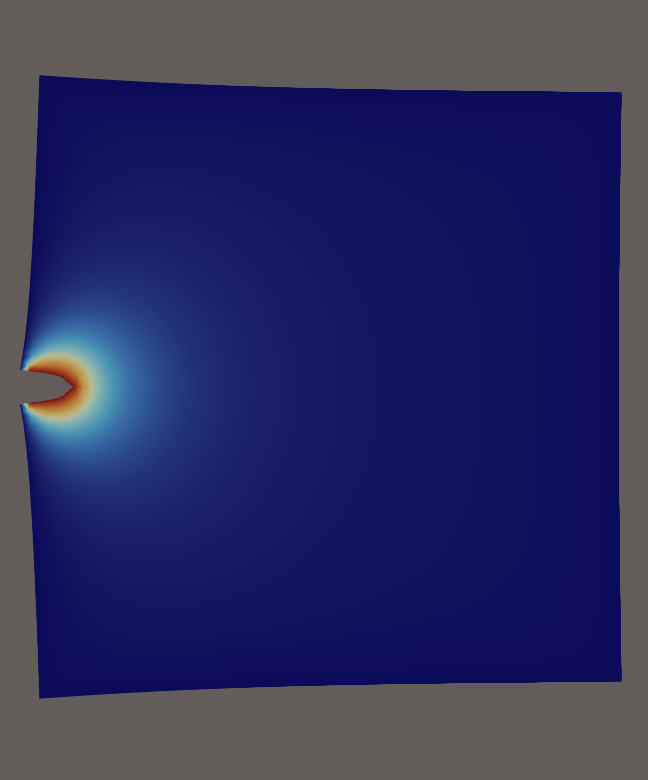
\includegraphics[width=0.3\textwidth]{output/PLOT_Surf_0.png}
	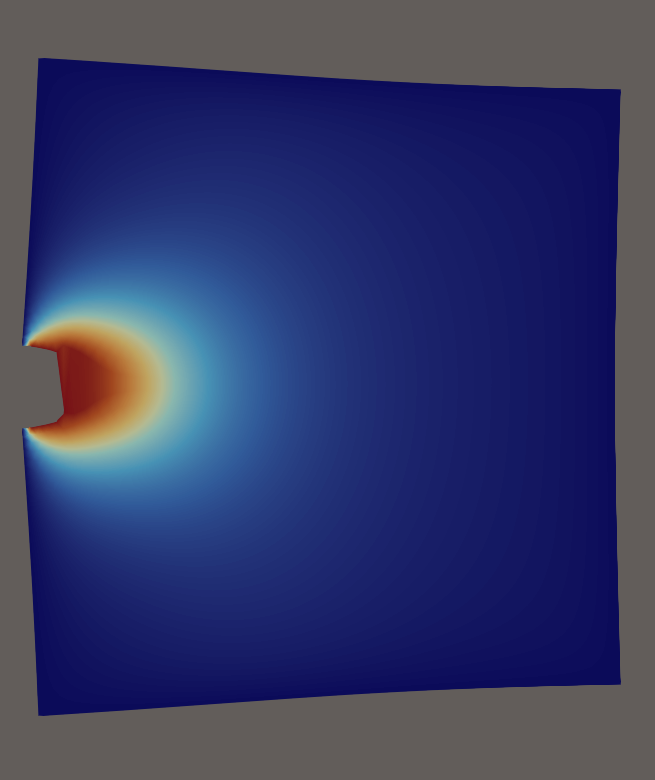
\includegraphics[width=0.3\textwidth]{output/PLOT_Surf_3.png}
	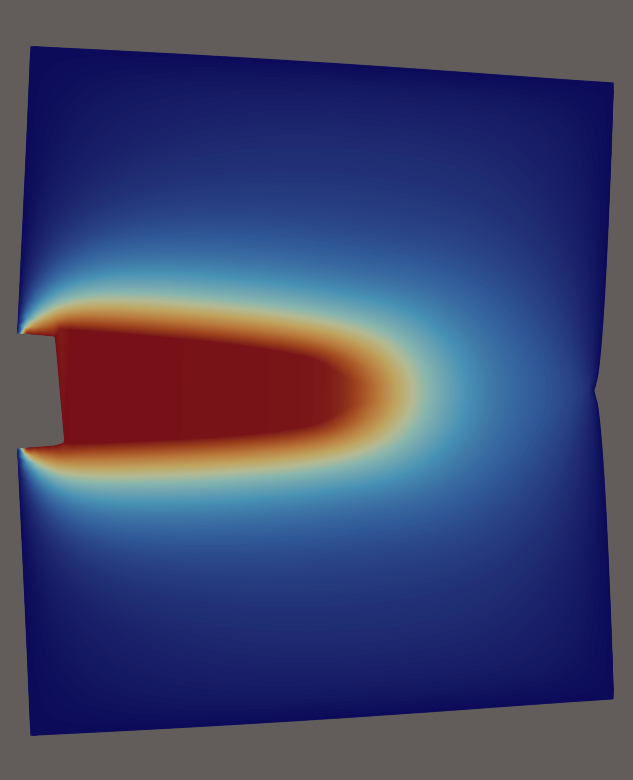
\includegraphics[width=0.3\textwidth]{output/PLOT_Surf_6.png}
	\caption{Crack progression of the surfing boundary conditions example.}
	\label{plot: surf}
\end{figure}
Figure \ref{plot: surf} shows the progression of the crack for this example.

\begin{figure}
	\centering
	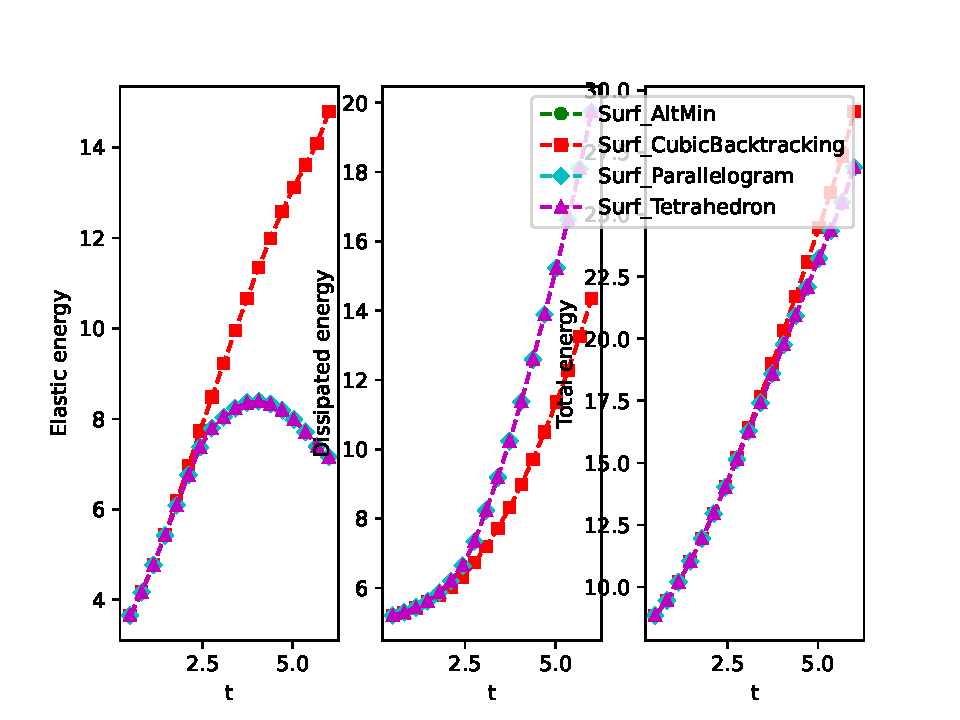
\includegraphics[width=100mm]{output/FIG_Surf_energy.pdf}
	\caption{Energy for the surfing example using the five methods tested.}
	\label{fig: surf energy}
\end{figure}
Figure \ref{fig: surf energy} shows the resulting energies produced by each of the five methods.
This can be used to determine correctness of the solutions.
We see that the elastic energy for the cubic backtracking continues to rise over all time steps, while for all other methods there is a point where it decreases.
Ultimately, the other four methods find lower total energy, and therefore produce more correct crack progression.

\begin{figure}
	\centering
	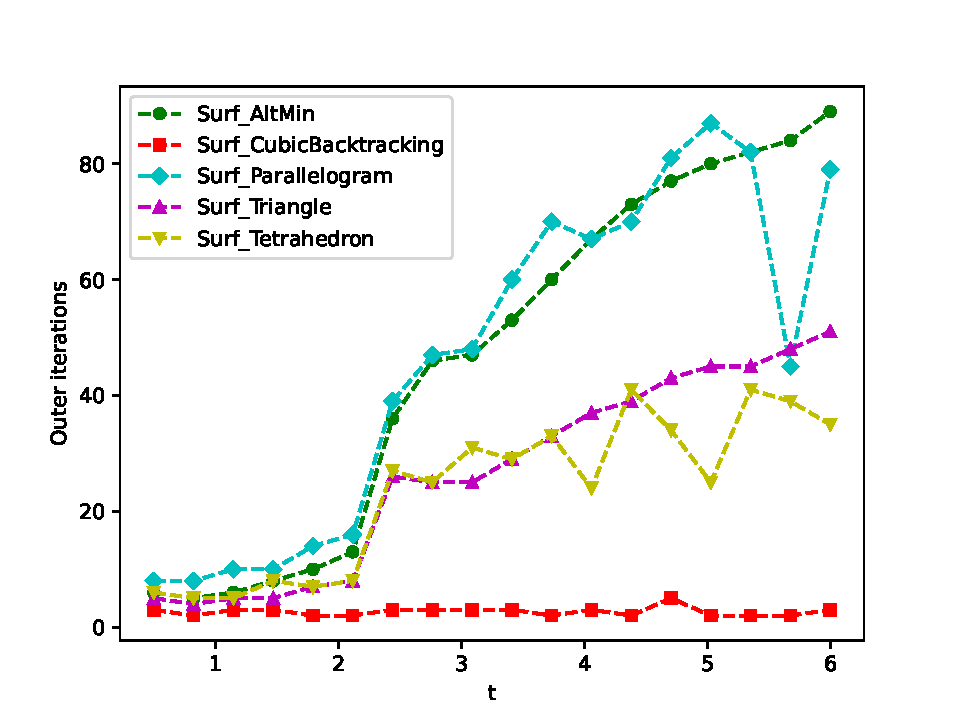
\includegraphics[width=100mm]{output/FIG_Surf_outerIts.pdf}
	\caption{Outer iterations (number of linear solves of the AltMin system) for each load step of the surfing example.}
	\label{fig: surf outer}
\end{figure}
Figure \ref{fig: surf outer} gives the number of outer iterations required for each load step to be completed for each of the five methods.
An outer iteration is characterized by a solve of the linear system defined by AltMin.
Cubic backtracking requires the lowest number of outer iterations, but we have seen that it produces the most problematic solution.
The three interpolant techniques require roughly half the number of outer iterations of AltMin.
The parallelogram and triangle interpolants behave about the same, while the tetrahedron performs marginally better.

\begin{figure}
	\centering
	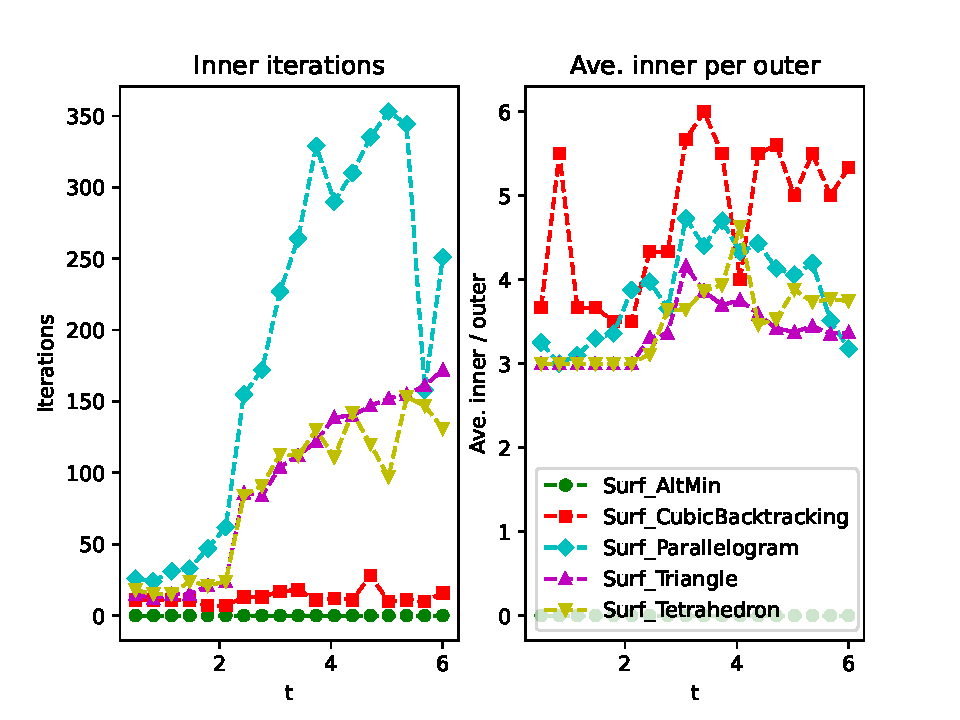
\includegraphics[width=100mm]{output/FIG_Surf_innerIts.pdf}
	\caption{On the left, total number of inner iterations (matrix-vector multiplications required to solve the Newton system to within tolerance) for the four methods that use inexact Newton.
	On the right, average number of inner iterations per outer iterations.}
	\label{fig: surf inner}
\end{figure}
Computation time is determined not only by the number of outer iterations, but also the number of inner iterations, a measure of the time to solve the inexact Newton step, see Figure \ref{fig: surf inner}.
However, the average number of inner iterations per outer iteration remains fairly constant for each method, meaning reducing the number of outer iterations remains the goal.
Cubic backtracking has a high average, at times over 5, while the three types of interpolants all remain between 3 and 4.

\begin{figure}
	\centering
	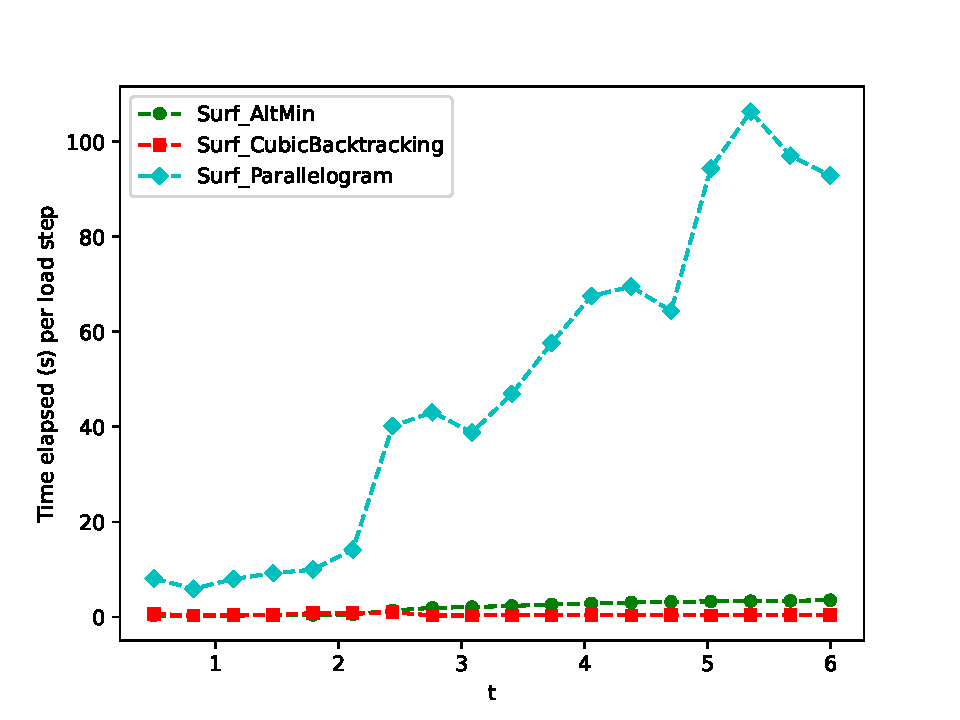
\includegraphics[width=100mm]{output/FIG_Surf_time.pdf}
	\caption{Wall clock time for solving the surfing example for all five methods.}
	\label{fig: surf time}
\end{figure}
Wall clock time includes several steps that can be avoided through code design, such as print statements and communication.
However, it gives some indication of the effectiveness of theoretical speedups.
Figure \ref{fig: surf time} gives the wall clock time for each of the five methods for each load step.
We see that AltMin has the best time of the accurate methods even though it requires the most number of outer iterations.
It is clear that care must be taken to reduce the number of flops spent on the inexact Newton step.

\begin{table}
	\centering
	\begin{tabular}{l | c c c}
	Method & Flops & \% AltMin & \% MSPIN \\ \hline
	AltMin & 3.970$\times 10^{10}$ & 99.9 \\
	Cubic backtracking & 1.538$\times 10^{10}$ & 43.6 & 56.3 \\
	Parallelogram & 5.178$\times 10^{10}$ & 45.9 & 53.7 \\
	Triangle & 5.175$\times 10^{10}$ & 45.8 & 53.9 \\
	Tetrahedron & 4.751$\times 10^{10}$ & 44.1 & 55.5
	\end{tabular}
	\caption{Flop count for the surfing example.}
	\label{tab: surf flops}
\end{table}
\begin{table}
	\centering
	\begin{tabular}{l | c c c}
	Method & Time (s) & \% AltMin & \% MSPIN \\ \hline
	AltMin & 3.583$\times 10^{1}$ & 64.3  \\
	Cubic backtracking & 1.946$\times 10^{1}$ & 22.6 & 14.9 \\
	Parallelogram & 3.963$\times 10^{1}$ & 35.2 & 23.4 \\
	Triangle & 3.905$\times 10^{1}$ & 35.9 & 23.8 \\
	Tetrahedron & 3.842$\times 10^{1}$ & 32.7 & 22.6
	\end{tabular}
	\caption{Timing for the surfing example.}
	\label{tab: surf time}
\end{table}
Table \ref{tab: surf flops} shows the number of flops for all five methods tested for the surfing example, while Table \ref{tab: surf time} gives the wall clock time for each.
Also shown is the percentage of flops and time spent completing the main computations: solving the linear system to compute the AltMin direction, and approximately solving the nonlinear system to compute the MSPIN direction.
These flop counts and timings are found using PETSc's built-in log view, and may be subject to errors.

While the MSPIN direction takes more flops to compute, it takes less time, likely due to better parallelization and preconditioning.
Since much of the MSPIN system has already been factorized during the solve of the AltMin direction, this factorization speeds up subsequent calculations.

We also note that approximately 40\% of time is spent on other tasks, though these tasks account for almost no flops.
This suggests communication issues arising from the parallelization, or wayward print statements.

\subsection{Three hole example}
\label{subsec: ctfm}

In this next example, we consider a rectangular domain with three holes, one large central hole and two smaller holes on either side.
A small notch starts the crack on the left edge, just above the level of the central hole.
Force is applied through the smaller holes in opposite directions, as if two rods are pulling the material apart.

Figure \ref{plot: ctfm} shows the progression of the crack for this example.
At a critical level of force, the crack propagates rapidly to the central hole.
If more force is applied, the crack will eventually nucleate on the right side of the central hole and propagate to the right edge, completely separating the material into two parts.
\begin{figure}
	\centering
	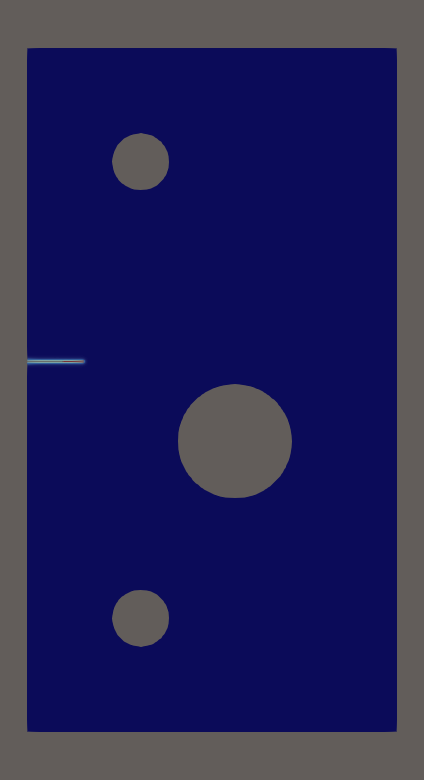
\includegraphics[width=0.3\textwidth]{output/PLOT_CTFM_0.png}
	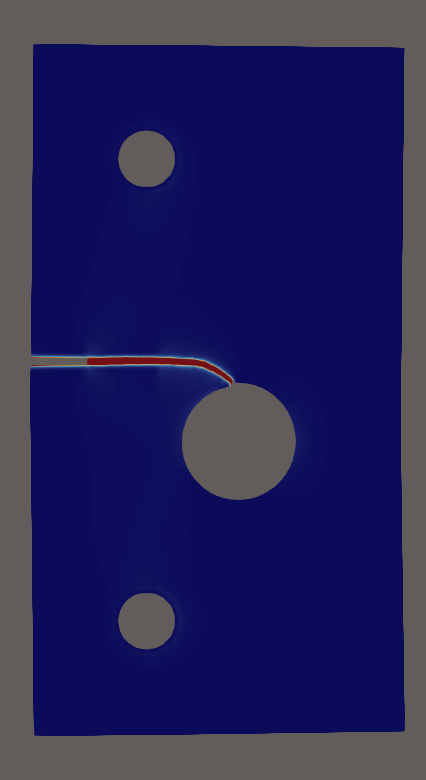
\includegraphics[width=0.3\textwidth]{output/PLOT_CTFM_0.5.png}
	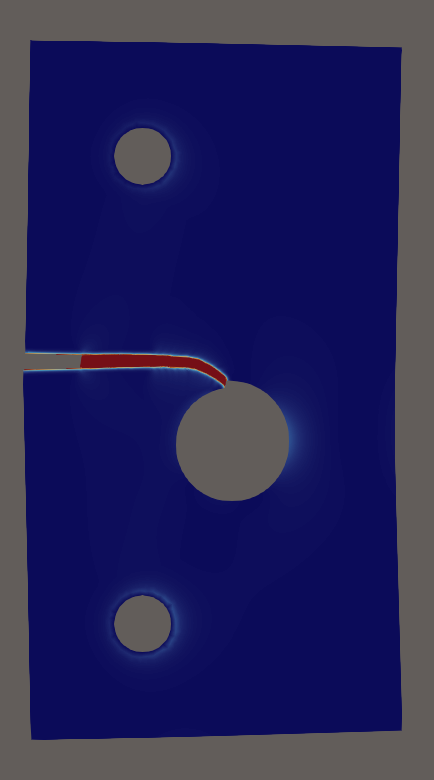
\includegraphics[width=0.3\textwidth]{output/PLOT_CTFM_1.png}
	\caption{Crack progression of the three hole example.}
	\label{plot: ctfm}
\end{figure}

\begin{figure}
	\centering
	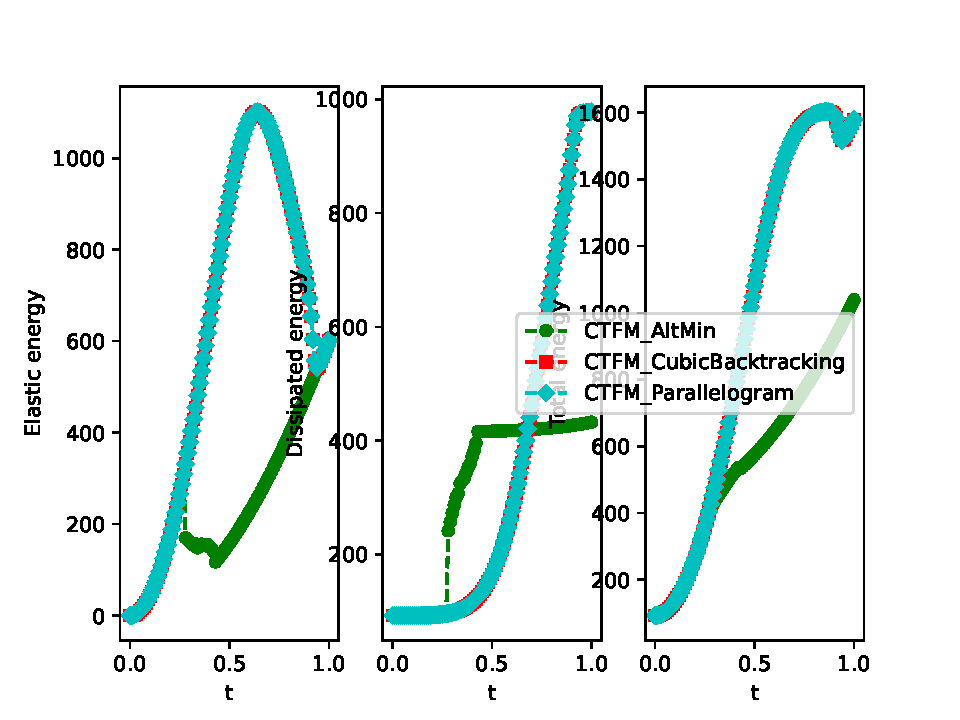
\includegraphics[width=100mm]{output/FIG_CTFM_energy.pdf}
	\caption{Energy for the three hole example using the five methods tested.}
	\label{fig: ctfm energy}
\end{figure}
Figure \ref{fig: ctfm energy} shows the resulting energies produced by the five methods.
As in the surfing example, the cubic backtracking is reticent to allow cracks to grow, instead preferring to increase elastic energy.
As the other four methods all have lower total energy potentials, their solutions indicate more appropriate crack progressions.

\begin{figure}
	\centering
	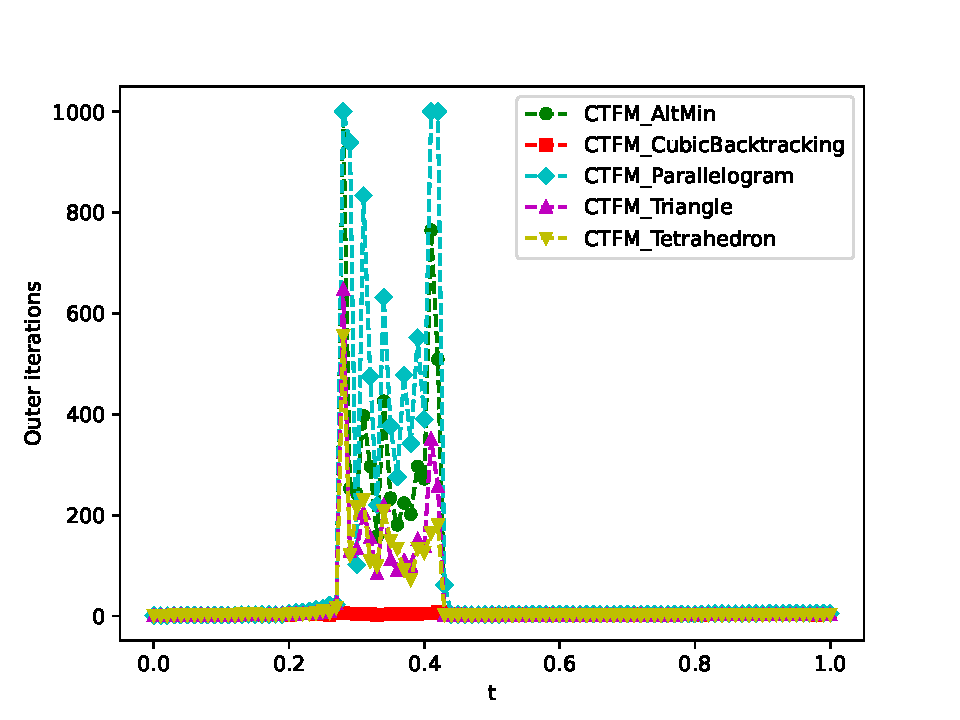
\includegraphics[width=100mm]{output/FIG_CTFM_outerIts.pdf}
	\caption{Outer iterations (number of linear solves of the AltMin system) for each load step of the three hole example.}
	\label{fig: ctfm outer}
\end{figure}
Figure \ref{fig: ctfm outer} gives the number of outer iterations required for the completion of each load step.
Each outer iteration represents the process of solving the linear system of AltMin.
Cubic backtracking again requires the lowest number of outer iterations, but at the expense of the highest potential energy.

The number of outer iterations only becomes significant for the load steps where the crack progresses rapidly.
In this regime, there are many ways for the crack to propagate that will result in lower energy, meaning the energy landscape has many saddle points and local minima.
Both the triangle and tetrahedron interpolants consistently have fewer outer iterations than AltMin.
The parallelogram interpolant is also often competitive, but not in a predictable way.

\begin{figure}
	\centering
	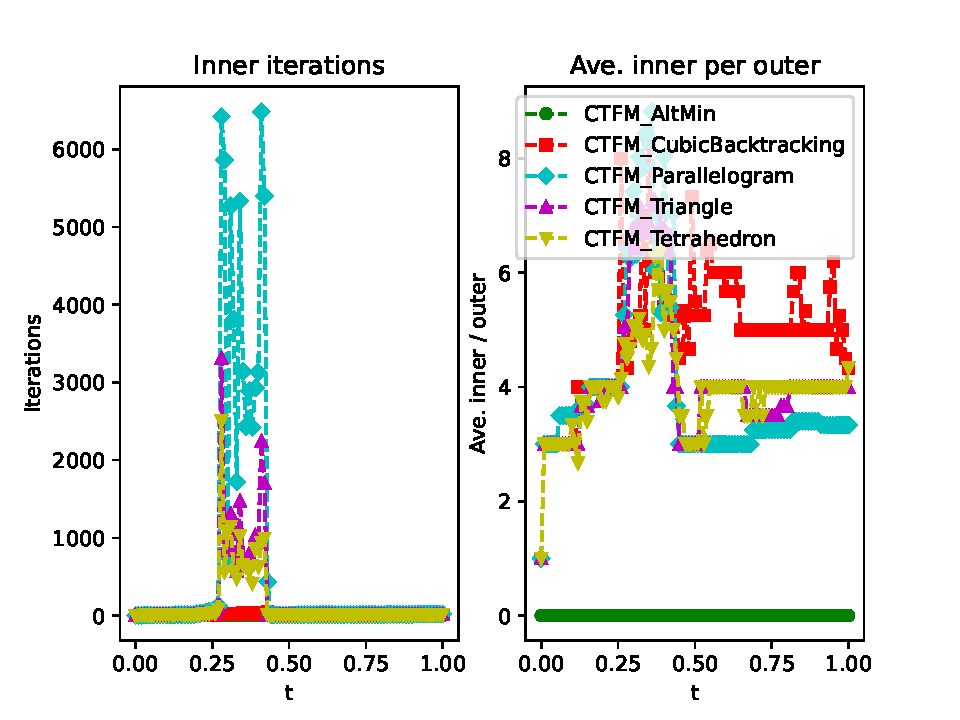
\includegraphics[width=100mm]{output/FIG_CTFM_innerIts.pdf}
	\caption{On the left, total number of inner iterations for the four non-AltMin methods.
		On the right, average number of inner iterations per outer iteration.}
	\label{fig: ctfm inner}
\end{figure}
Figure \ref{fig: ctfm inner} shows the additional cost of the MSPIN-based methods over AltMin:
the number of matrix-vector multiplications required to solve the inexact Newton problem.
The number of inner iterations is closely correlated with the number of outer iterations performed.
However, the average number of inner iterations per outer iteration spikes during the crack propagation regime, suggesting the MSPIN system becomes more complicated to resolve at this stage.

\begin{figure}
	\centering
	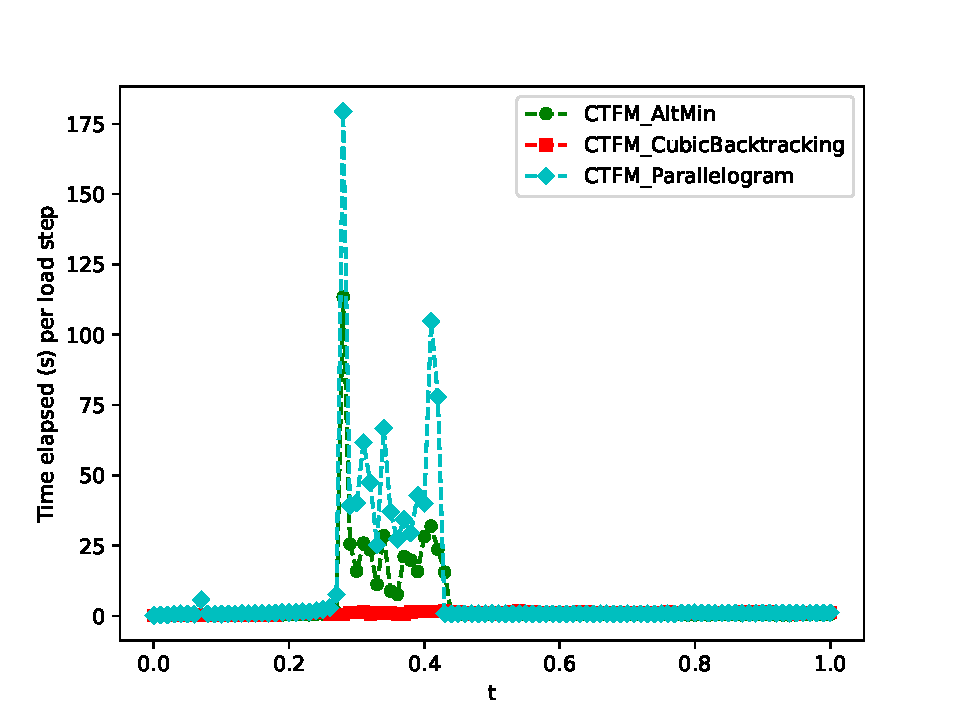
\includegraphics[width=100mm]{output/FIG_CTFM_time.pdf}
	\caption{Wall clock time for each load step for the three hole example.}
	\label{fig: ctfm time}
\end{figure}
Figure \ref{fig: ctfm time} gives a measure of the amount of time each method takes to complete each load step.
As expected, most time is spent during the crack propagation regime.
AltMin and the triangle and tetrahedron interpolants take roughly the same amount of time, with the parallelogram interpolant struggling due to its high number of outer iterations.

\begin{table}
	\centering
	\begin{tabular}{l | c c c}
	Method & Flops & \% AltMin & \% MSPIN \\ \hline
	AltMin & 1.160 $\times 10^{14}$ & 100 \\
	Cubic backtracking & 2.196 $\times 10^{13}$ & 36.8 & 63.1 \\
	Parallelogram & 5.631 $\times 10^{14}$ & 32.4 & 67.6 \\
	Triangle & 1.744 $\times 10^{14}$ & 36.6 & 63.4 \\
	Tetrahedron & 1.670 $\times 10^{14}$ & 35.0 & 65.0
	\end{tabular}
	\caption{Flop count for the three hole example.}
	\label{tab: ctfm flops}
\end{table}
\begin{table}
	\centering
	\begin{tabular}{l | c c c}
	Method & Time (s) & \% AltMin & \% MSPIN \\ \hline
	AltMin & 1.321 $\times 10^3$ & 96.7 \\
	Cubic backtracking & 2.760 $\times 10^2$ & 35.3 & 48.9 \\
	Parallelogram & 5.893 $\times 10^3$ & 33.7 & 64.2 \\
	Triangle & 2.066 $\times 10^3$ & 38.2 & 58.3 \\
	Tetrahedron & 1.871 $\times 10^3$ & 35.7 & 60.5
	\end{tabular}
	\caption{Timings for the three hole example.}
	\label{tab: ctfm time}
\end{table}
Table \ref{tab: ctfm flops} gives the number of flops for each method on this example, while Table \ref{tab: ctfm time} gives the timings.
Both tables include the percentage of each measure that is spent on the linear and nonlinear solves.
The difference in costs between linear and nonlinear solves here is much more stark than in the previous example, with the nonlinear solves costing nearly twice as much as the linear solves in terms of both flops and time.
This suggests a lack of scalability in the preconditioning methods used to speed up the MSPIN calculations.

It is clear that using MSPIN with the interpolant minimization techniques can reduce the number of outer iterations, often significantly.
However, doing so greatly increases the computational cost of each outer iteration, up to 290\%.
To be competitive against AltMin, the number of outer iterations will need to be reduced by a factor of 3.

\end{document}